\documentclass[aspectratio=169]{beamer}
\setbeamertemplate{navigation symbols}{}
\usepackage{color,amsmath,comment, subfigure}
\usepackage{booktabs}
\def\vf{\vfill}
\usepackage{url}

%\setbeameroption{show notes}

%%%%%%%%%%%%%%%%%%%%%%%%%%
\title[]{Class 10: Thresholds, cascades, and predictability}
\author[]{Matthew J. Salganik}
\institute[]{Sociology 204: Social Networks\\Princeton University}
\date[]{
2/2 Threshold model on networks
\vfill
\begin{flushleft}
\vspace{0.6in}
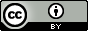
\includegraphics[width=0.1\textwidth]{figures/cc.png}
\end{flushleft}

}

\begin{document}
%%%%%%%%%%%%%%%%%%%%%%%%%%%
\frame{\titlepage}
%%%%%%%%%%%%%%%%%%%%%%%%%%%
\begin{frame}

Now what happens when people following a threshold rule are placed into a network? What kinds of cascades can occur?
\pause

\begin{center}
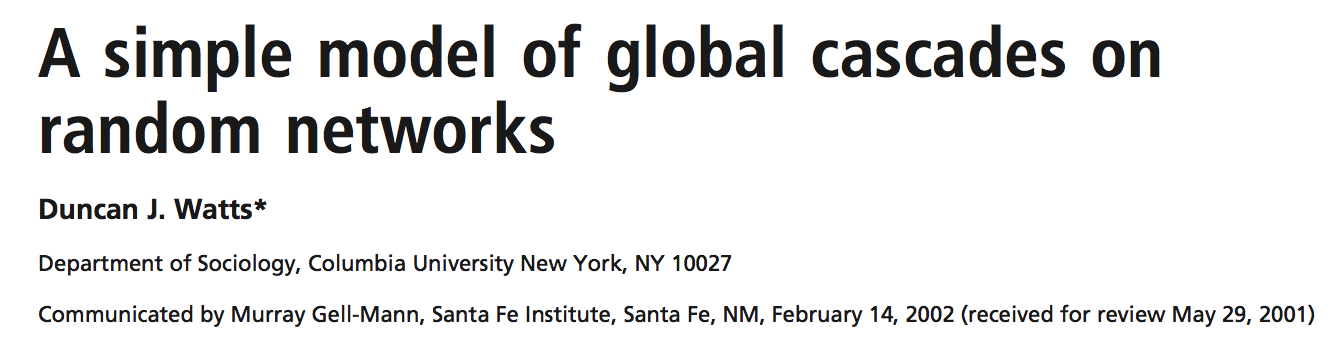
\includegraphics[width=0.9\textwidth]{figures/watts_simple_2002_title}
\end{center}

\vfill
Simple model of individual behavior + simple network $\rightarrow$ complex collective behavior

\end{frame}
%%%%%%%%%%%%%%%%%%%%%%%%%%%%
\begin{frame}

Setup:
\begin{itemize}
\item Homogenous thresholds on Erdos-Reyni random graph
\item All nodes turned off
\item One node randomly turned on
\end{itemize}
\pause

\only<2>{\includegraphics[width=0.6\textwidth]{figures_book/8_4}}
\only<3>{\includegraphics[width=0.6\textwidth]{figures_book/8_5}}


\note{
Explain phase diagram, what is x-axis, what is y-axis.  

Also, the shape of the diagram is not intuitive.  You should not obviously see why it is this shape.  If this is clear, come talk to me.

Why is this phase diagram stair-stepy (for lack of a better word)?  This is related to the number of neighbors on can have and still be vulnerable.  When average threshold goes from 0.21 to 0.19 someone with a degree of 5 can become vulnerable.  When threshold goes from 0.17 to 0.16 someone with degree of 6  can become vulnerable and so on.\\

In the cascade window there are percolating clusters of vulnerables

Forest fire: Not about the spark, about the environment

Think-pair-share:
Pick a point inside cascade window.  Imagine that you are President Eisgruber and you want to prevent a riot.  What are the strategies you could use?  State them in abstract terms and concrete terms.

}
\end{frame}
%%%%%%%%%%%%%%%%%%%%%%%%%%%
\begin{frame}

Note that the percolating vulnerable cluster is not about influential people; it is about easily influenced people

\end{frame}
%%%%%%%%%%%%%%%%%%%%%%%%%%%
%\begin{frame}
%
%\begin{center}
%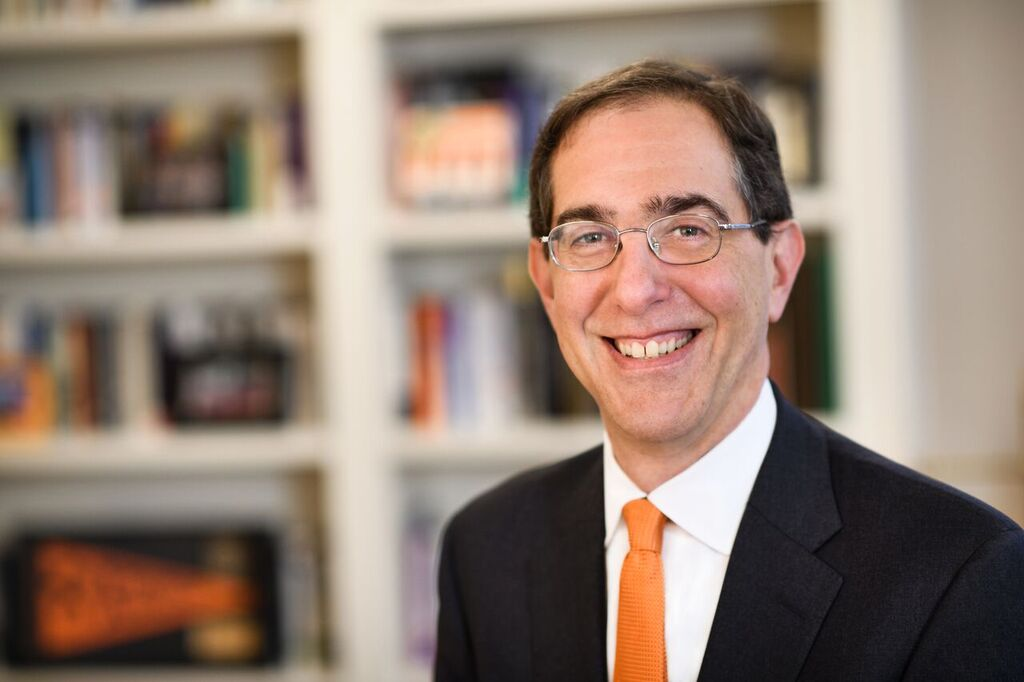
\includegraphics[width=0.6\textwidth]{figures/eisgruber}
%\end{center}
%I need your help.
%
%How can I prevent the riots?
%
%\vfill
%\tiny{\url{http://www.princeton.edu/president/eisgruber/who/eisgruber/Indoor.jpg}}
%
%\end{frame}
%%%%%%%%%%%%%%%%%%%%%%%%%%%
%\begin{frame}
%
%Assume:
%\begin{itemize}
%\item the social network of Princeton students is an Erdos-Renyi random graph
%\item all Princeton students have exactly the same threshold
%\end{itemize}
%\pause
%What do you recommend? 
%\vfill
%\begin{center}
%\includegraphics[width=0.5\textwidth]{figures_book/8_5}
%\end{center}
%\pause
%\vspace{-0.45in}
%Many approaches.  Change connectivity or change thresholds. If you change connectivity, you can decrease the chance of riots by either decreasing or increasing connectivity.
%\end{frame}
%%%%%%%%%%%%%%%%%%%%%%%%%%%
\begin{frame}

Assumes: Homogenous thresholds on Erdos-Reyni random graph (Watts 2002 calls it ``uniform random graph'').  What about heterogeneity?

\end{frame}
%%%%%%%%%%%%%%%%%%%%%%%%%
\begin{frame}

Heterogeneity in thresholds makes cascade window bigger.

\begin{center}
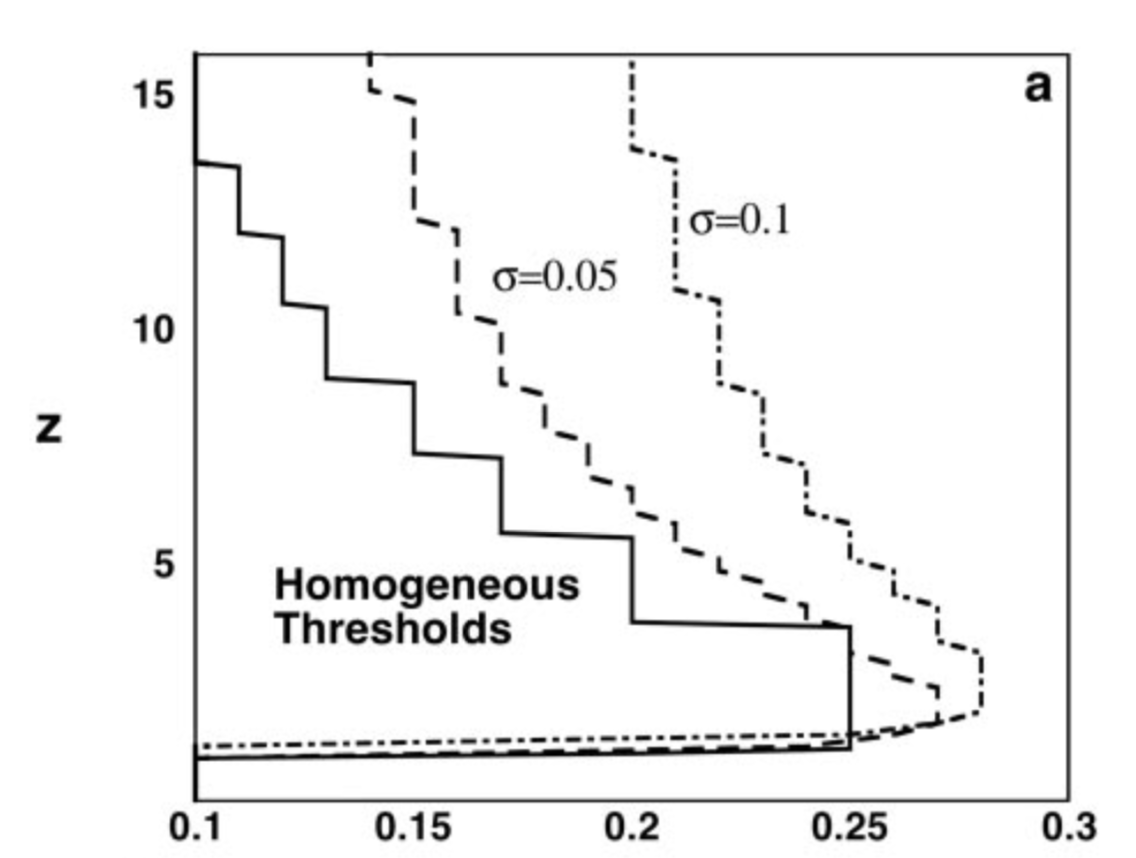
\includegraphics[width=0.5\textwidth]{figures/watts_simple_2002_fig4a}
\end{center}

\end{frame}
%%%%%%%%%%%%%%%%%%%%%%%%%
\begin{frame}

Heterogeneity in degree distribution makes cascade window smaller.

\begin{center}
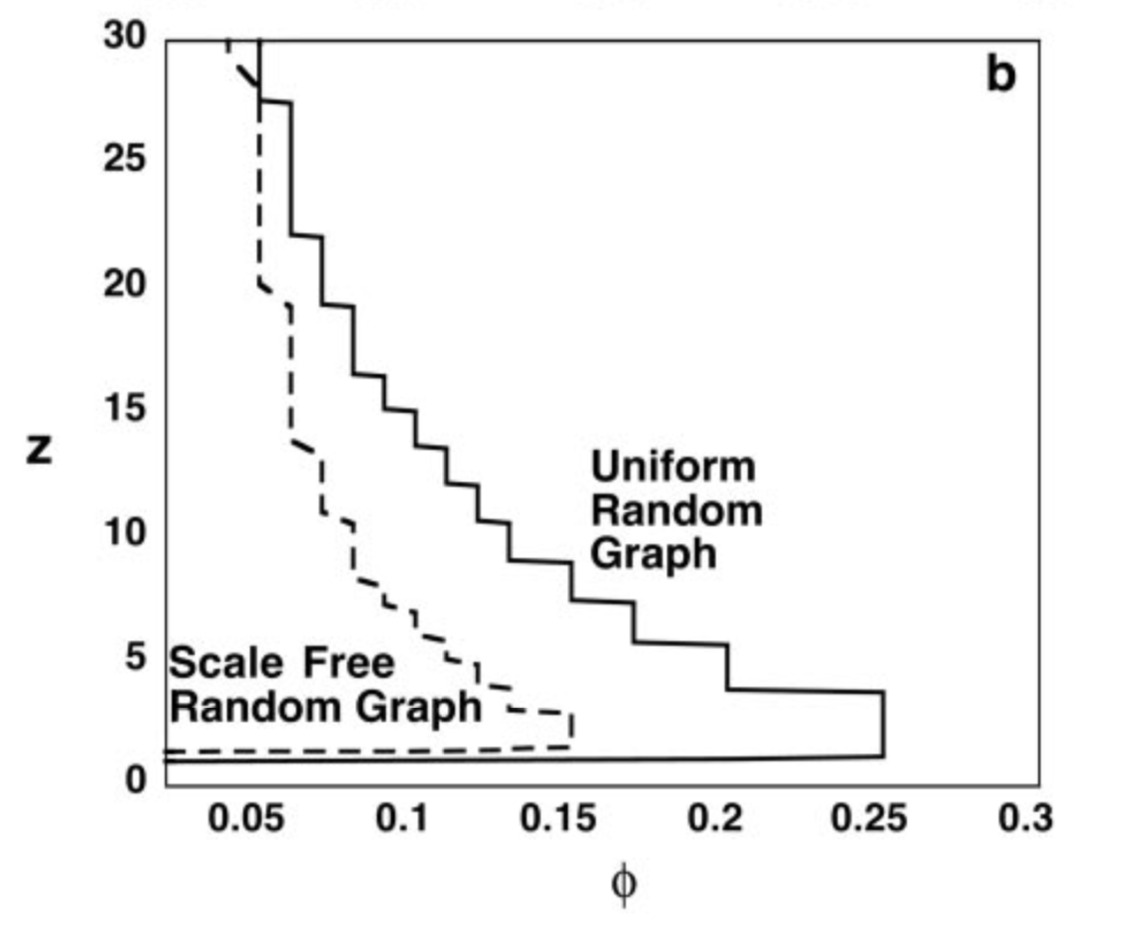
\includegraphics[width=0.5\textwidth]{figures/watts_simple_2002_fig4b}
\end{center}

\end{frame}
%%%%%%%%%%%%%%%%%%%%%%%%%
\begin{frame}

\vspace{-0.6in}
\begin{center}
\includegraphics[width=0.5\textwidth]{figures_book/8_5}
\end{center}
\vspace{-0.4in}
Think back to the comparison of biological and social contagion.
\begin{itemize}
\item \onslide<1->In biological contagion what is the effect of increased connectivity? \onslide<2->{\textcolor{green}{More spread}}
\item \onslide<3->In social contagion what is the effect of increased connectivity? \onslide<4->{\textcolor{green}{It depends}}
\end{itemize}

\note{

Gladwell was wrong :)

}

\end{frame}
%%%%%%%%%%%%%%%%%%%%%%%%%%%
\begin{frame}

Model in Watts (2002) helps us understand why
\begin{itemize}
\item global cascades can be triggered by very small shocks
\pause
\item global cascades occur rarely despite many shocks that are a priori indistinguishable
\end{itemize}

\end{frame}
%%%%%%%%%%%%%%%%%%%%%%%%%%%
\begin{frame}

\begin{center}
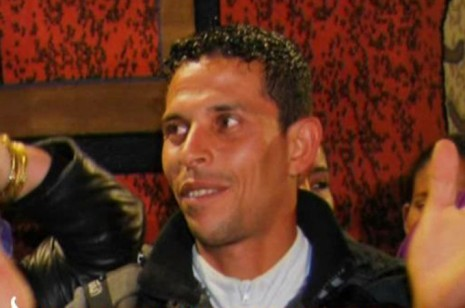
\includegraphics[width=0.8\textwidth]{figures/Mohamed_Bouazizi}
\end{center}
Mohamed Bouazizi

\vfill
\tiny{\url{http://en.wikipedia.org/wiki/File:Mohamed_Bouazizi.jpg}}

\note{

Mohamed Bouazizi sets himself on fire

}

\end{frame}
%%%%%%%%%%%%%%%%%%%%%%%%%%%
\begin{frame}

\begin{center}
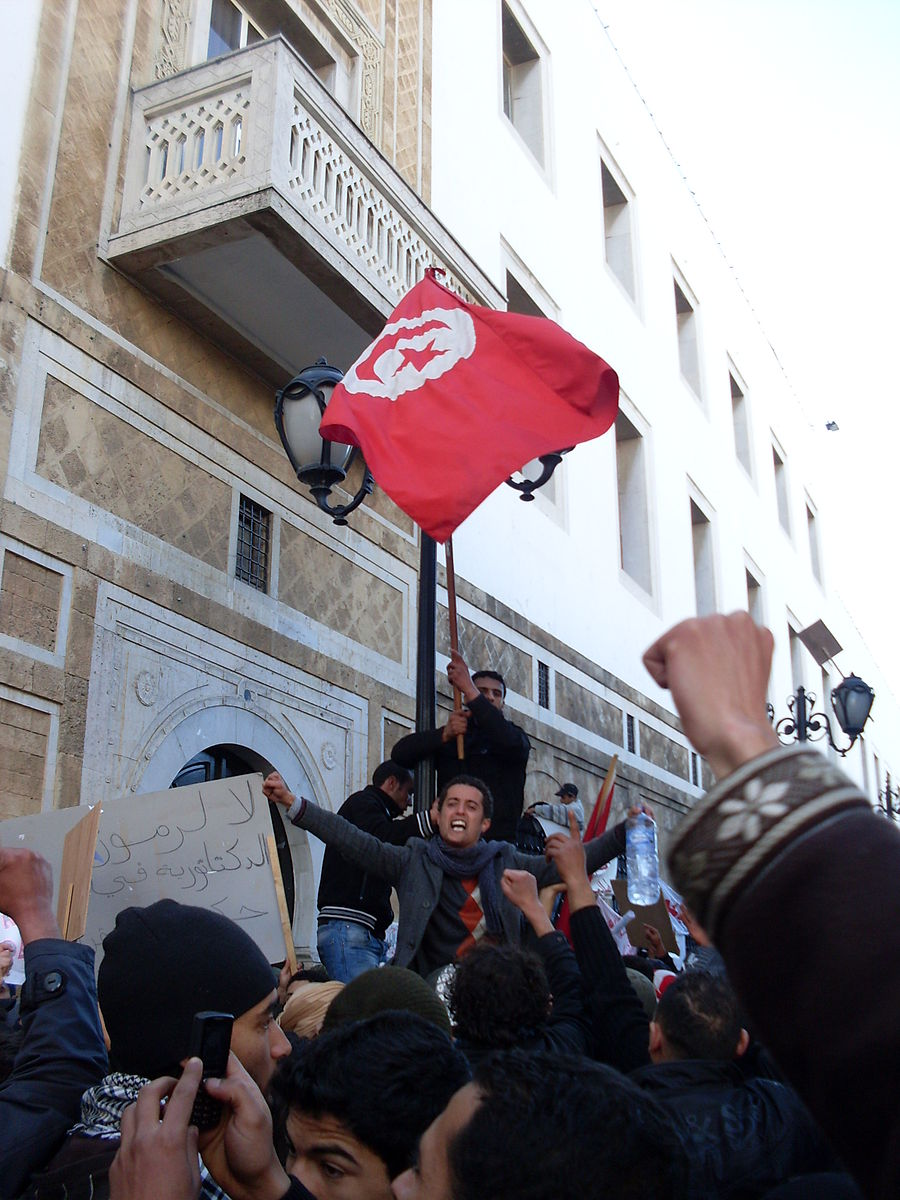
\includegraphics[height=0.8\textheight]{figures/tunisia_protests}
\end{center}

\tiny{\url{http://commons.wikimedia.org/wiki/File:Caravane_de_la_lib\%C3\%A9ration_4.jpg}}

\note{
Protests rock Tunisia
}

\end{frame}
%%%%%%%%%%%%%%%%%%%%%%%%%%%
\begin{frame}

\begin{center}
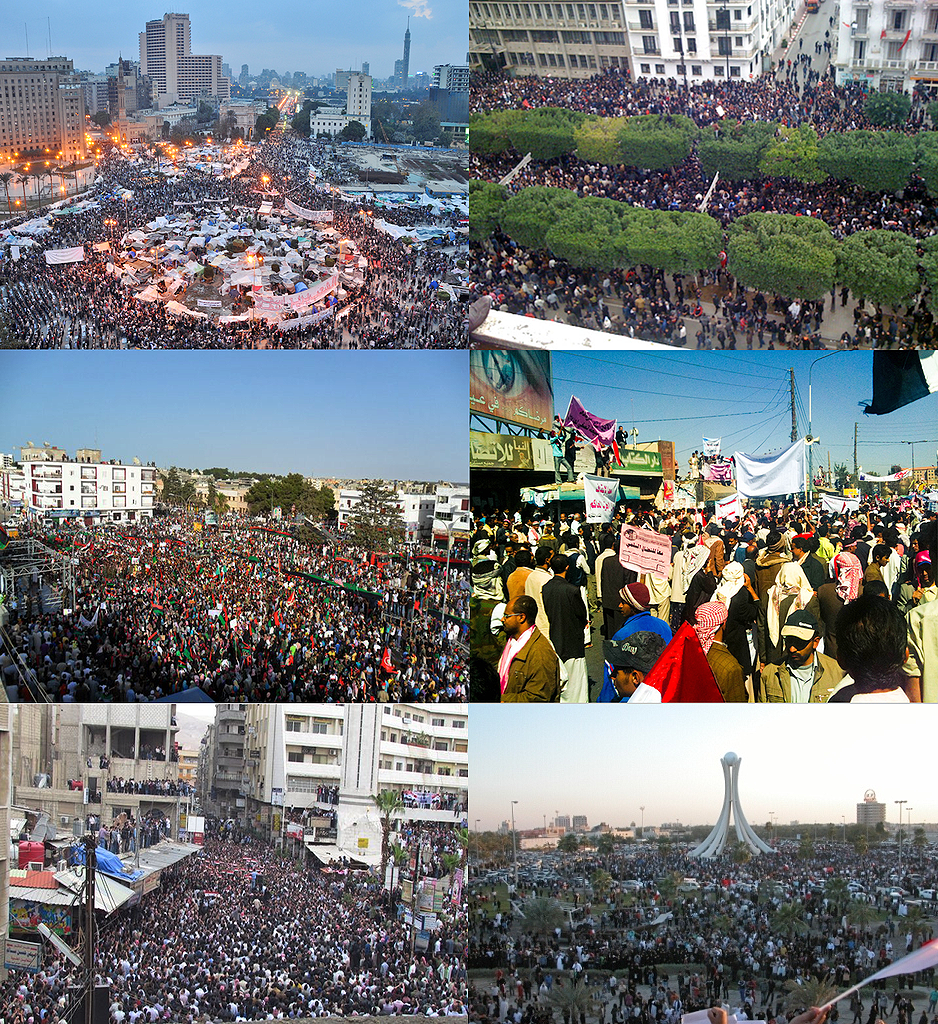
\includegraphics[height=0.8\textheight]{figures/arab_spring}
\end{center}

\tiny{\url{http://commons.wikimedia.org/wiki/File:Info_box_collage_for_mena_Arabic_protests.png}}

\note{

Clockwise from top left:
\begin{itemize}
\item Egypt
\item Tunisia
\item Yemen
\item Bahrain
\item Syria
\item Libya
\end{itemize}
When we see a big event we want to figure out who started it.  Is Mohamed Bouazizi special?  Maybe that's not thee right way to think about it.  

}

\end{frame}
%%%%%%%%%%%%%%%%%%%%%%%%%%%
\begin{frame}

Summary:
\begin{itemize}
\item disease contagion and social contagion have different micro rules and macro dynamics
\pause
\item hard to predict collective outcome from individual preferences and hard to infer individual preferences from collective outcomes
\pause
\item sometimes small shocks get big and sometimes they don't
\end{itemize}

\end{frame}
%%%%%%%%%%%%%%%%%%%%%%%%%%%
\begin{frame}

Next class:
\begin{itemize}
\item Hedstrom, P. (2006). Experimental macro sociology: Predicting the next best seller. \textit{Science}.
\item Salganik, M.J., Dodds, P.S., and Watts, D.J. (2006). Experimental study of inequality and unpredictability in an artificial cultural market. \textit{Science}.
\item Salganik, M.J., and Watts, D.J. (2008). Leading the herd astray: Experimental study of self-fulfilling prophecies in an artificial cultural market. \textit{Social Psychology Quarterly}.
\end{itemize}


\end{frame}
%%%%%%%%%%%%%%%%%%%%%%%%%%

\end{document}
